\chapter{Contribution}

As stated in previous section, IIDEAA is a set of newly developed tools that has not been used widely. It is crucial to test out IIDEAA thoroughly to detect possible bugs and identify current limitations of the framework so that further improvement can be made. In this testing phase, we used projects from AxBench, a benchmark designed for Approximate Computing, to see whether both tools of IIDEAA can work properly. Additionally, since one of the ambitions for IIDEAA is to apply Approximate Computing techniques to certain Artificial Neural Network libraries, compatibility with these libraries is also an issue to address. The two library that were tested are DarkNet and Fast Artificial Neural Network(FANN). \\
~\\
The last objective of this internship is to create a new tool to generate Approximate variants based on the results of the 2 other tools. However, due to visa issues, the internship was delayed, thus having less time for it than intended. Because of this, we have only started to work on and scratched the surface of this matter.\\

\section{Testing Environment}

It is worthwhile to discuss about the environment used to conduct all tests with IIDEAA. In this framework, both Chimera and Bellerophon required LLVM-3.9.1, which was an older version of this compiler tools (current version is 7.0.0). Other than that, Bellerophon needs ParadisEO to be installed, because it uses the engine for Evolution Searching, as pointed out in the last chapter. Ideally, we would like to install everything in a separate machine for conveniences in testing, debugging and modifying the source code. However, installing LLVM was a difficult task and we ran into many problems. Luckily, The developer of the framework has provided us with the option of using a Docker image. This image was based on the ArchLinux default image and has everything needed for IIDEAA to run seemlessly.\\
\vspace*{3cm}

\section{Evaluating and Debugging IIDEAA}

\subsection{Applying IIDEAA to AxBench's benchmark}

AxBench is a benchmark containing a set of applications used for various approximate computing research. The benchmark was written in C++ and has some typical applications from various domain such as finance, image processing, signal processing to investigate different aspects of Approximate Computing \cite{7755728}. The benchmark comes in with implemetations for both CPU and GPU. For the sake of simplicity, we've chosen to use CPU-based applications to validate IIDEAA. \\
~\\
Aside from providing configuration files with desired parameters to Chimera and Bellerophon, in order to use the sample projects from AxBench with IIDEAA, additions and modifications have to be made to these projects. First is the inclusion of a CMake auto-config file for each project. CMake is a tool designed to build, test and package software that can generate Makefile for C/C++ project automatically, which is convenient for the programmer. An important note when configuring the project using CMake is that generating a \textit{compile\_command.json} is necessary. This is due to the fact that both Chimera and Bellerophon will use it later on for syntax check and compilation. For Bellerophon case, some modifications needs to be made to make sure that the compiler has the correct path to the mutated files. \\
~\\
As mentioned in chapter 2, the user has to define how to calculate the error causes by precision loss and the reward gained from this loss to Bellerophon. Since the error metrics for each AxBench project were made public by the development team, we have used them to implement the error function. As for the reward function, it depends on how the Approximate Operator works. For this testing phase, we used two Operators implemeted by IIDEAA's developer, VPA and VPA\_Native. The two Operators are designed for Precision Scaling strategy as they modify the precision/data type. The reward function regarding these two Operators will be discussed in the \textit{Result and Discussion} section. \\
~\\
In addition, source code modification sometimes is required to ensure that Bellerophon will have a function that can be called to execute the main part of the program, thus producing the approximated result for each variation of the mutated program. Lastly, the user must also have a \textit{.txt} file containing the result produced by the original version of the program. Because the source code of the program is the mutated one, it is more convenient to read the original result from the text file. Also, since the comparision between both versions, original and mutated, is made for every variant, having the original source ran repeatedly is time consuming. \\
~\\
All the projects that were setup to be able to run by IIDEAA are available at: \url{https://github.com/nnkhoa/IIDEAA-Bench}. \\

\subsection{Bugs encountered}

While testing IIDEAA with project from AxBench, we have found a few unwanted behaviors resided in the framework, the major ones being a few cases of incorrect mutation from Chimera caused by inaccurate interpretation of the source code's Abstract Syntax Tree. Another bug found was due to overlooking type casting in calculation while mutating, thus causing ambiguity when calling parameterized constructor as the object may not have constructor implemented for arguments in such data types. \\
~\\
To demonstrate bugs regarding the mutation process, consider the following example: 
\begin{minted}[fontsize=\normalsize]{cpp}
	#define DIV 1.5
	#define TEST(X, Y) (X + Y)
	
	int k, N;
	float r;			float x, y, z;
	
	/*
	 * initialize value for the variables
	 */
	
	r =   x/y; /*(1)*/	r = (float) k/N; /*(2)*/
	r = x/DIV; /*(3)*/	r = TEST(x, y) + z; /*(4)*/
\end{minted}
The correct behavior can be expected when mutating calculation (\textit{1}) is as follow:
\begin{minted}[fontsize=\normalsize]{cpp}
	r = (float) ::vpa::VPA(x, OP_1)/::vpa::VPA(y, OP_2);
\end{minted}
In general, the mutation process will travel down the Abstract Syntax Tree, searching for specific Tree Nodes that contain paticuliar symbols, depending on the definition of the Mutation Operator. For example, in the case of VPA\_Native Operator, Chimera will look for any Binary Operators or Binary Assign Operators such as add and subtract. Once these operators are found, Chimera will attempt to make modifications on the left hand side and/or right hand side of the operator based on the API of the Approximate Operator. \\
\begin{figure}[H]
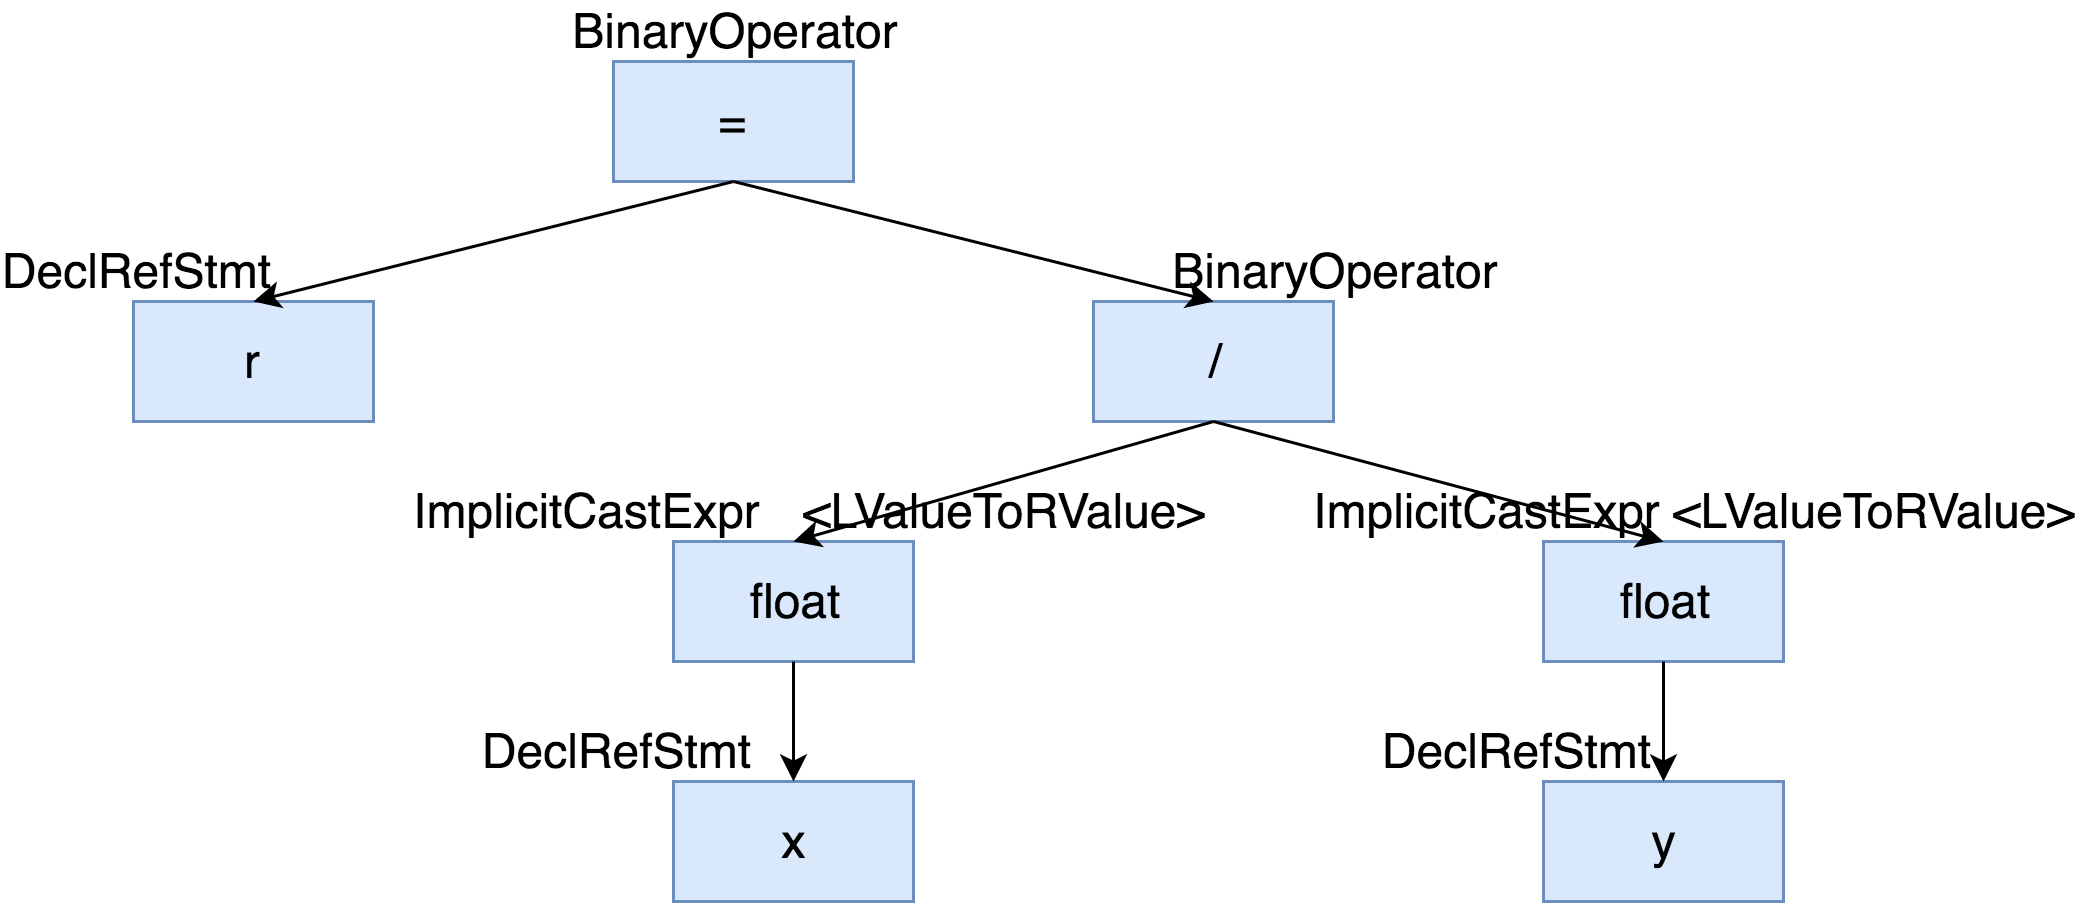
\includegraphics[width=12cm]{AST-1.png}
\centering
\caption{AST (1) Analysis with Chimera}
\end{figure}
~\\
From the above mutation, the \verb|VPA| constructor from the VPA\_Native approximate operator takes in 2 arguments. The first one is variable of either the following type: \textit{float}, \textit{double}, \textit{long double}. The second one contains the information about the precision to be changed when execute Bellerophon. \\
~\\
However, when mutating calculation (\textit{2}), while the mutation was correct as intended from the developers, it still caused errors during compilation:
\begin{minted}[fontsize=\normalsize]{cpp}
	fatal error: call to constructor of ::vpa::VPA is ambiguous
	r = (float)((float) ::vpa::VPA(k, OP_1)/::vpa::VPA(N, OP_2));
						^
\end{minted}
To breifly explain, in (\textit{2}), the C-Style cast was applied to make sure the result of the division \textit{k/N}, which is the division of 2 \textit{integer},is of the same type with \textit{r} (\textit{float}, in this case). However, Chimera did not consider the this type of cast and just mutated the calculation normally as if there was nothing out of the ordinary. Thus, it caused a "confusion" to the compiler as VPA\_Native did not have any constructor for integer variable. \\
\begin{figure}[H]
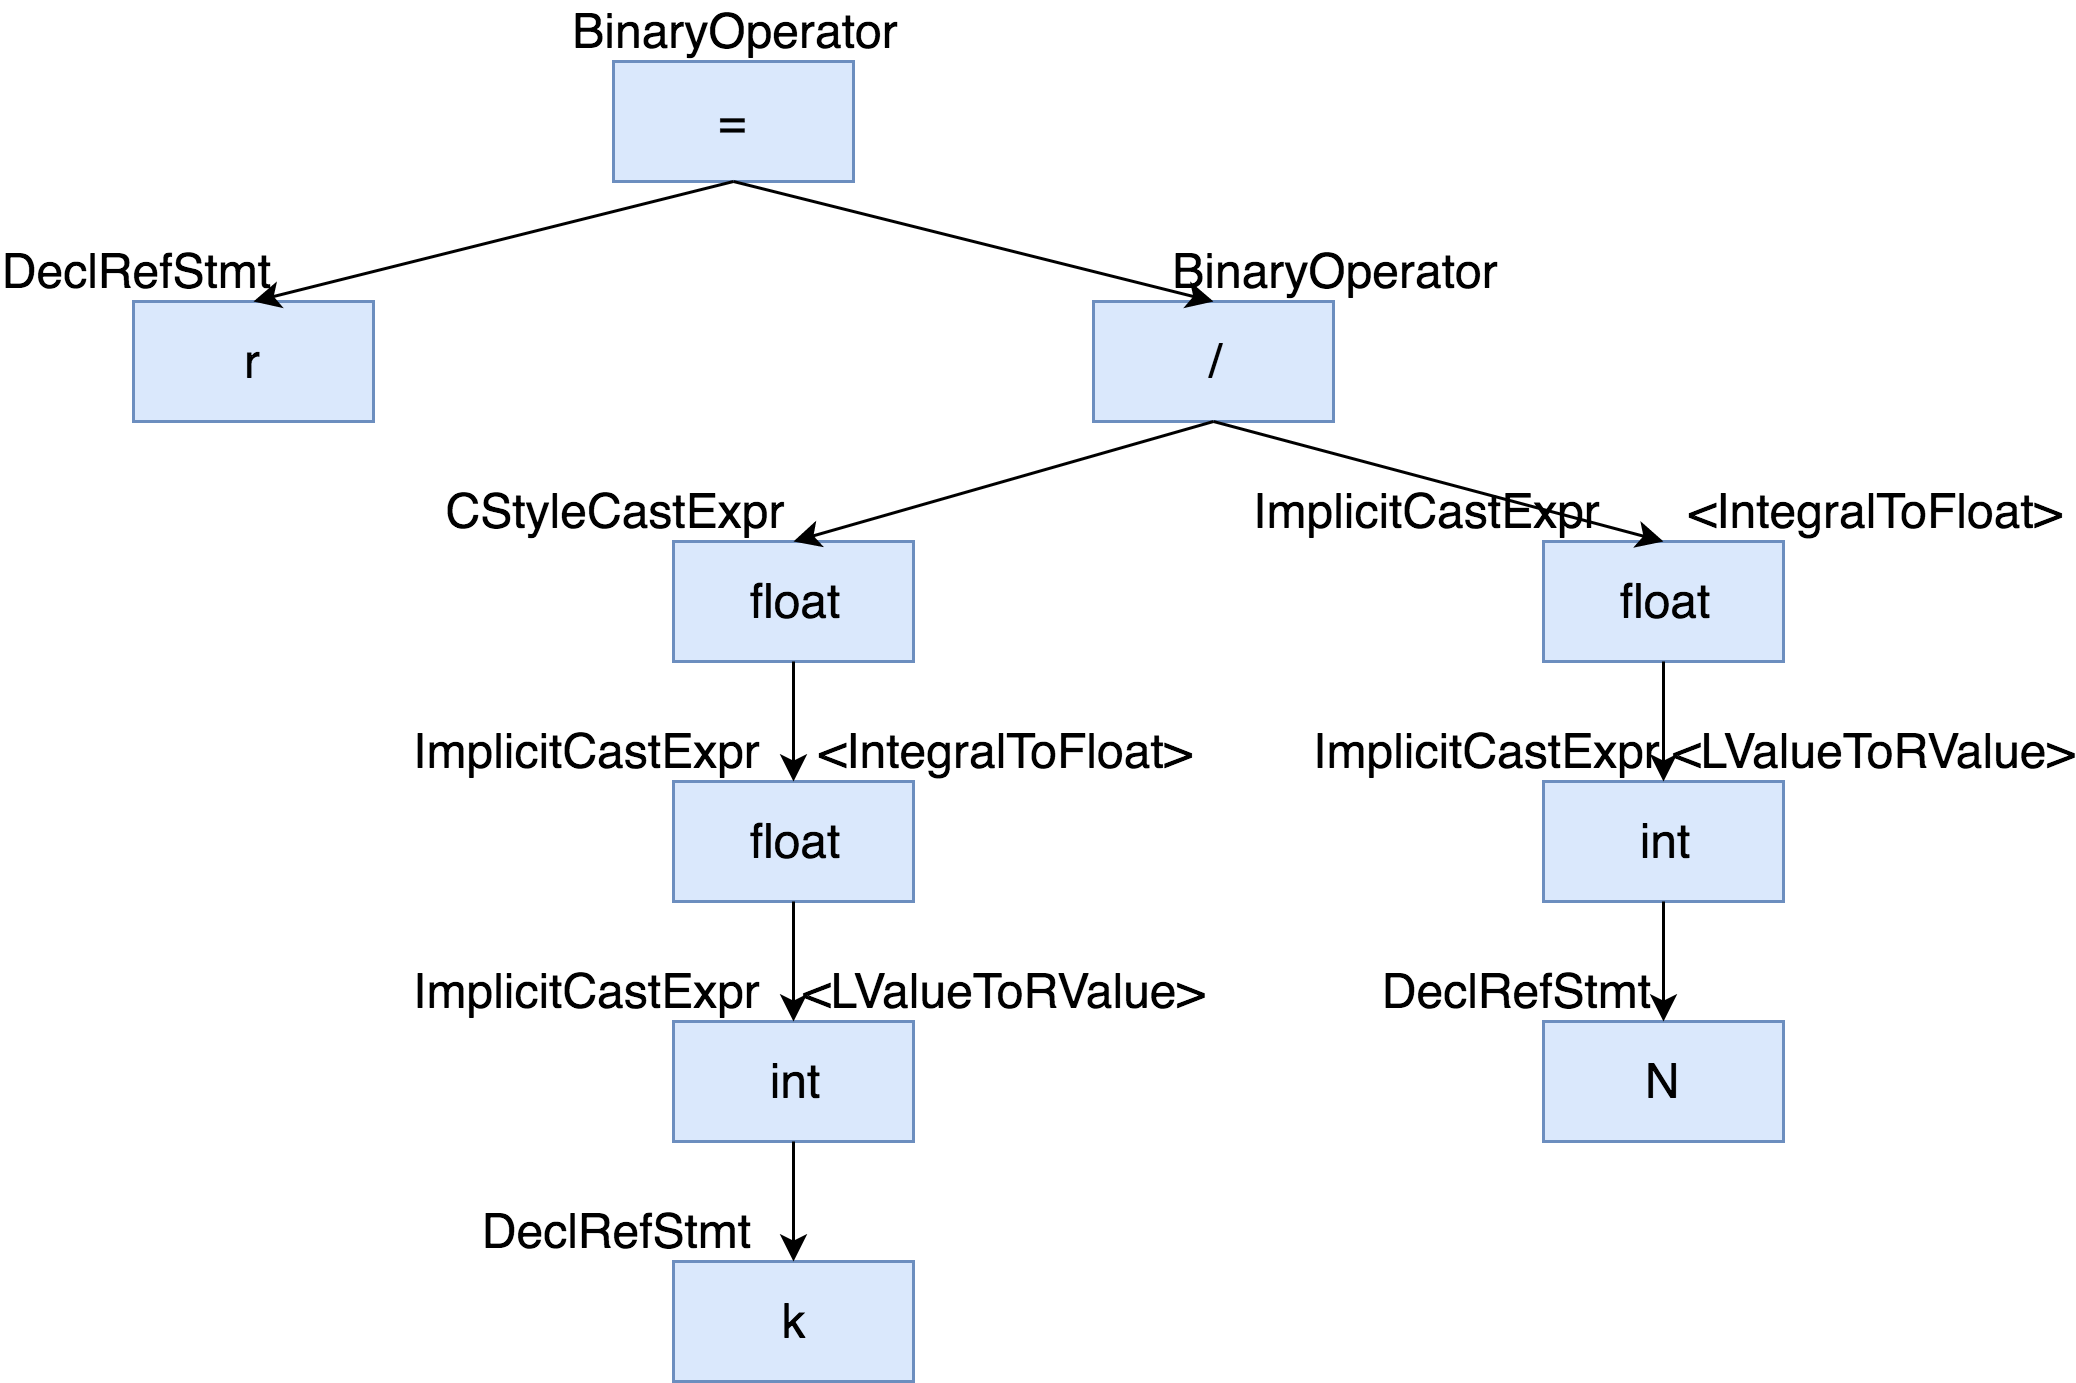
\includegraphics[width=12cm]{AST-2.png}
\centering
\caption{AST (2) Analysis with Chimera}
\end{figure}

~\\
In the case of (\textit{3}) and (\textit{4}), since \textit{DIV} and \textit{TEST} are macros, they were not counted as either variablse or functions, and were not properly handled, thus causing errors as below when the mutation is complete:
\begin{minted}[fontsize=\normalsize]{cpp}
	// calculation number 3
	fatal error: expected ')'
        r =(float)( ::vpa_n::VPA(x , OP_0)/ DIV;
        									   ^
	note: to match this '('
        r =(float)( ::vpa_n::VPA(x , OP_0)/ DIV;
                        ^

	// calculation number 4
	fatal error: assigning to float from incompatible type vpa_n::VPA
        r =(float)( TEST(x, y) , OP_1) +::vpa_n::VPA( z, OP_1));
          ^~~~~~~~~~~~~~~~~~~~~~~~~~~~~~~~~~~~~~~~~~~~~~~~~~~~
\end{minted}
As can be seen, the mutation finished incorrectly as there are some missing syntaxes and parenthesis compared to the normal behavior. When we tried to extract and analyze information from the Abstract Syntax Tree of these calculations, fetching names of these macros, according to the position to the Binary Operator, returned empty, thus making the Mutator had nothing to base on and did not perform any mutation. However, the Abstract Syntax Tree still recognized that these are macros. This may be reason why the mutation process ended up being incorrect. \\
\begin{figure}[H]
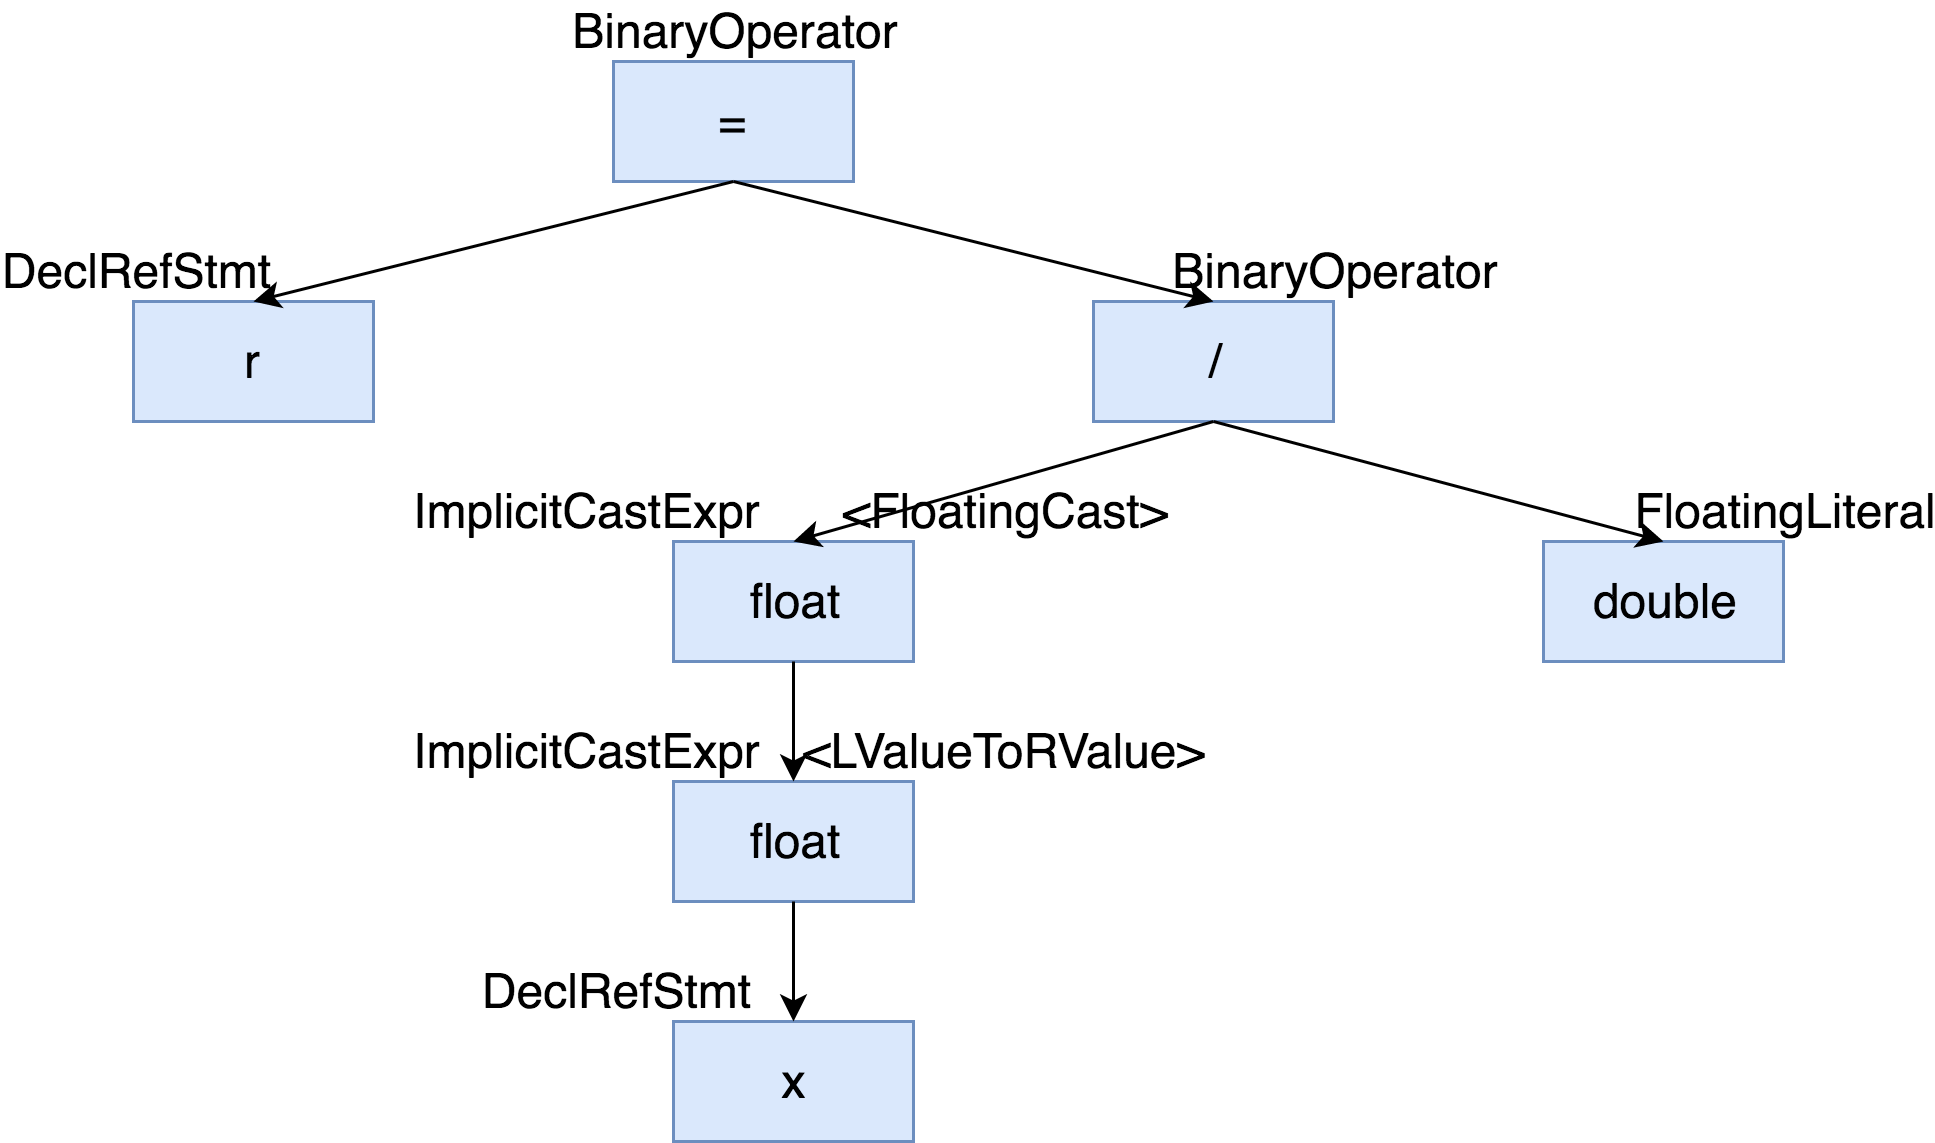
\includegraphics[width=12cm]{AST-3.png}
\centering
\caption{AST (3) Analysis with Chimera}
\end{figure}
~\\
There are other undesired behaviors which led to program crashes, not due to the actual source code of the framework, but because of incompatability between project's dependencies and testing environment. For example, in the \textit{Sobel} project from AxBench, it is required that the system should have \textit{Boost Library} installed. However, compilation using the library was not sucessful due to versions mismatch of a depedency named \textit{icu}, which is a core component of ArchLinux Docker image. Updating this component will require a full update of the current system. However, after the update, we experienced that this has interfered with the functionality of ParadisEO and inherently, Bellerophon, making them unusable. \\

\subsection{Analyzing and Debugging}

For the problems regarding Chimera, analyzing and understanding how the Abstract Syntax Tree works is the one way to approach these issues. With the problem of C-Style cast with calculations that concern different data types, to avoid simillar problems in the future, we assumed that the variables used in the calculation all have different data types to the casting type. Because of this, we made sure that if there is any cast of the previously-mentioned type that is detected during the mutation process, we will mutate each varible, applying casts to these variables before further mutation. \\
\begin{algorithm}[H]
\SetAlgoLined
\KwResult{Detect C-Style Cast and Mutate Accordingly}
$lhs \leftarrow getLeftHandSide(BinaryOperator)$\;
$rhs \leftarrow getRightHandSide(BinaryOperator)$\;
$cast \leftarrow getCast(lhs)$\;
Mutation Process\;
\If{cast NOT null}{
	\If{cast.isCStyle()}{
		applyCast(rhs, cast)\;
	}	
}
Continue Mutation Process\;
\caption{Dealing with C-Style Cast in mutation}
\end{algorithm}
~\\
This approach will ensure that even if the constructor does not have any implemetation for the data type, everything will still work as expected. The result of the mutation after debugging for (\textit{2}) is as below
\begin{minted}[fontsize=\normalsize]{cpp}
	r = (float)(::vpa::VPA((float)k, OP_1)/::vpa::VPA((float)N, OP_1));
\end{minted}
Another way to deal with this problem is to modify the Approximate Operator library to have support for at least all basic data types. However, sometimes the intention is to only include an implentation for certain data types, depending on the purpose of the Approximate Operator. \\
~\\
The problem of (\textit{3}) and (\textit{4}) was a bit tricky to debug on account of the fact that some information returned by the AST was missing. In the case of (\textit{3}), as the macro was only a Literal Value, we followed the same principle as we did on the previous problem, performing check for appearances of \textit{Macro} and \textit{Literal} statement classes, then perform mutation accordingly. The same, however, could not be applied to (\textit{4}) because this was a function-like Macro with arguments which made debugging difficult, especially when the information returned from the Abstract Syntax Tree was missing. Currently, we do not have any solution for this problem so we try to avoid using projects or parts of the project that contains this Pre-processor. The best we can do is to try and replace these function-like Macros with proper functions. \\
\begin{algorithm}[H]
\SetAlgoLined
\KwResult{Mutate correctly code with Literal Value Macro}
$lhs \leftarrow getLeftHandSide(BinaryOperator)$\;
$rhs \leftarrow getRightHandSide(BinaryOperator)$\;
Mutation Process\;
\If{lhs.hasMacro()}{
	\If{Macro.isLiteral()}{
		Mutate Accordingly\;
	}	
}
\If{rhs.hasMacro()}{
	\If{Macro.isLiteral()}{
		Mutate Accordingly\;
	}	
}
Continue Mutation Process\;
\caption{Dealing with Literal Value Macro in mutation}
\end{algorithm}
~\\
The debugged version of Chimera can be found at: \url{https://github.com/nnkhoa/clang-chimera}.\\

\section{Compatibility with Artificial Neural Network libraries}

In this phase, the goal is to verify that IIDEAA can be used with some of the existing Artificial Neural Network libraries. Preferably, we try to find libraries that are open-source and required the least amount of dependencies. Due to the issues with the run-time environment stated in the previous chapter, a library that was implemented in pure C++ and without the need for external library would be the most suitable for the current iteration of IIDEAA. Libraries that are compatible with IIDEAA should not encounter any trouble during run-time of both Chimera and Bellerophon.\\

\subsection{Darknet}

Darknet\cite{darknet13} is a neural network framework written purely in C and has CUDA extension for some GPU applications. It was developed and still being updated by Joseph Redmon. With this framework, the programmer is able to develop many artificial neural network-related applications, from simple image classification programs to sophisticated applications such as playing a game of GO or running real-time object detection.\\
~\\
We have chosen this particuliar framework because it matches our criteria of being available open-source while not having to rely on external libraries. We've tried to apply IIDEAA to Darknet, however it was not very successful. The problem was due to the old infrastructure of LLVM that Bellerophon is using. For that particuliar version, the Just-In-Time compiler of Clang was unable to handle the assembly code that was implemented within a crucial Darknet library for image loading/encoding from file/memory, thus crashing the program. This is another drawback of IIDEAA that needs to be addressed since LLVM has been updated steadily for the past few years. \\
~\\
The framework is available at: \url{https://github.com/pjreddie/darknet}.\\

\subsection{Fast Artificial Neural Network(FANN)}

Fast Artificial Neural Network\cite{fann}, also known as FANN for short, was developed by Steffen Nissen's team and have been updated regularly for the past 10 years. This library is implemented purely in C, having support for backpropagation multilayer network that can be either fully or sparsely connected. Along with the library, the team also provides a handful of examples to demonstrate its simplicity, versatility and speed, which was declared by the author to be up to 150 times faster, in terms of execution, than other libraries. \\
~\\
To test this library against IIDEAA, we used an pre-existing example called mushroom, a mushroom classification that determines whether a mushroom is edible or not based on large number of the mushroom's characteristics. This example was based on the PROBEN1 benchmark, a collection of neural network benchmark problems that represent realistic problems. The mushroom dataset has 125 inputs that describe the mushroom features such as shape, color, fragrance, but only has 2 outputs and it is one of the easier example that was given by the development team. \\
~\\
Since the mushroom example uses backpropagation neural network, choosing which part of the library to Approximate should also be considered. Backpropagation usually contains 5 phases: provide input, network feed-fowarding, output error calculation, error backpropagation, and calculate output. Currently, we've tried to aim at approximate the error backpropagation phase since it is a crucial part of Backpropagtion Neural Network and we wanted to see how much Approximate Computing can affect it. The mutate operator used in this experiment was the \textit{VPA} operator. Result of evaluating FANN will be discussed in the next chapter.\\
~\\
While the desired \textit{MSE}(shorts for \textit{Mean Square Error}) after training of this classification was set to 0.00001 just like the default setting, \textit{epoch}, which indicates the number of full training cycle on the training set, was reduced from 300 to only 50 cycles. This is due to 2 reasons. The first being that the original version of the example usually takes less than 20 cycles to reach the preferred \textit{MSE}. Secondly, after observing Bellerophon explored approximated versions, we found that having 300 full cycles of training was redundant since doing so did not improve the network significantly, if at all, and was very time-consuming given that there were many variants of the network to be executed. \\
~\\
Aside from the reward function that remained the same as those of previous tests, we had included a penalty which is used for calculating the time it would take to finish the execution of each variant of the neural network. To be specific, this metric considered the actual training time of the network. In terms of validating the error caused by the Approximation, we chose to compare the differences between the result of mutated versions and the original to see how much they deviate from each other in the validating phase. The threshold for a result to be sufficient was no more than 0.00002, which was double of the \textit{MSE} of the original version.\\
~\\ 
FANN code base can be found at: \url{https://github.com/libfann/fann}.\\